\section{初边值问题}
\label{sec:heat-ibvp}

取一根长度为$1$的细棒，中点加热到$1/2$度，向两端线性降到$0$度，初始温度就是一个三角形鼓包
\begin{equation}
 u_0(x)=\min\{x,1-x\},\qquad 0\leq x\leq 1 .
 \label{eq:heat-tent}
\end{equation}
棒的侧面包着隔热层，只有两端可能与外界交换热量。松手之后温度怎样变化？回答它需要一个方程，还需要说清初始时刻和两端发生了什么。

\paragraph{局部守恒与Fourier定律}
先看棒上任意一段$[a,b]$。记$u(x,t)$为温度，选取单位，使单位长度的棒升高一度所需的热量为$1$，于是这一段含有的热量是$\int_a^bu\,\mathrm{d}x$。再记$q(x,t)$为单位时间向右穿过截面$x$的热量，$f(x,t)$为单位长度、单位时间内产生的热量。

如图~\ref{fig:heat-bar-balance}，这一段热量的变化只有三个来源：从左端流入，从右端流出，内部产生。写成等式是
\[
 \frac{\mathrm{d}}{\mathrm{d}t}\int_a^bu\,\mathrm{d}x=q(a,t)-q(b,t)+\int_a^bf\,\mathrm{d}x .
\]

\begin{BookInlineFigure}
  \centering
  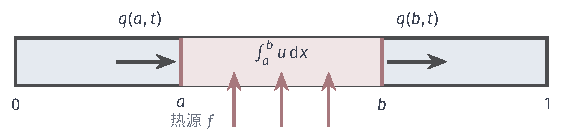
\includegraphics[width=96mm]{figures/06-differential-equations/02-partial-differential-equations/tikz/heat-bar-balance/figure.pdf}
  \caption{细棒上一段$[a,b]$（红色浅底）的热量收支。左右两个箭头是穿过截面的热流$q$，向右为正；下方红色箭头是内部热源$f$。段内热量的变化率等于流入减流出再加内部产生。}
  \label{fig:heat-bar-balance}
\end{BookInlineFigure}

这个等式对任何传递机制都成立，它有$u$和$q$两个未知量，还不能决定演化。补上的一条是物质的性质：热量从高温流向低温，流量正比于温度的斜率，这称为\term{Fourier定律}（Fourier's law）：
\[
 q=-\kappa\,\partial_xu ,
\]
其中$\kappa>0$是导热能力。斜率为正时右边更热，$q<0$，热量向左流，符号正好如此。

设$u$足够光滑。由微积分基本定理，$q(a,t)-q(b,t)=-\int_a^b\partial_xq\,\mathrm{d}x$。把它和Fourier定律代入收支等式，并把对$t$的导数移进积分，得到
\[
 \int_a^b\bigl(\partial_tu-\kappa\,\partial_x^2u-f\bigr)\,\mathrm{d}x=0 .
\]
这对每一段$[a,b]$都成立。被积函数连续，若它在某点不为零，就在一小段上保持同号，取这一小段作$[a,b]$，积分不为零，矛盾。所以被积函数处处为零，即
\begin{equation}
 \partial_tu=\kappa\,\partial_x^2u+f .
 \label{eq:heat-1d-kappa}
\end{equation}
这就是\term{扩散方程}（diffusion equation），在温度的语境下称为\term{热方程}（heat equation）。

\paragraph{向邻居的平均值靠拢}
二阶导数比较的是一点与邻点的平均。由Taylor展开，
\[
 \partial_x^2u(x,t)\approx\frac{2}{h^2}\Bigl(\frac{u(x-h,t)+u(x+h,t)}{2}-u(x,t)\Bigr) .
\]
于是无源时，每一点的温度变化率正比于“邻居平均值减自己”。比邻居平均值高的地方降温，低的地方升温，这就是抹平。

拿式~\eqref{eq:heat-tent}的三角形来看。在两条直线段上，邻居的平均值恰好等于自己，这些点一开始不想变化；只有中点比邻居的平均值高，所以降温从峰顶开始，再逐渐向两侧传开。下面图~\ref{fig:heat-bump-two-boundaries}中最浅的一条曲线正是这样：直线段的大部分还贴着初值，峰顶已经被削圆。

\paragraph{尺度与多维形式}
系数$\kappa$和棒长都可以通过选单位消去。设棒长为$L$，令$x=Ly$、$t=(L^2/\kappa)s$，代入无源方程，得到$\partial_su=\partial_y^2u$。所以时间的自然单位是$L^2/\kappa$：棒长加倍，抹平到同样程度要四倍的时间。这个平方关系后面还会以$\sqrt{t}$的形式反复出现。

高维的推导相同，把截面换成任意小区域的边界，用散度定理把边界通量变成体积分。材料各向异性时通量是$-\bm{A}(\bm{x})\nabla u$，方程是$\partial_tu=\nabla\cdot(\bm{A}\nabla u)+f$，其中$\bm{A}$对称且一致正定。本章取$\bm{A}=\bm{I}$，一维时即$\kappa=1$，这样可以把全部注意力放在解的结构上。

\paragraph{初值、热源与边界}
一个方程不足以确定温度，还要指定开始时的状态和区域边缘的情况。下面把问题写完整，$\Omega\subset\mathbb{R}^{d}$是有界开集，$T>0$。

\begin{definition}[初边值问题]
\label{def:heat-ibvp}
给定源项$f$、初值$u_0$和边界数据$g$，扩散方程的\term{初边值问题}（initial-boundary value problem）是求$u(\bm{x},t)$，使得
\begin{equation}
 \begin{aligned}
  \partial_tu&=\Delta u+f, && \bm{x}\in\Omega,\ 0<t\leq T,\\
  u(\bm{x},0)&=u_0(\bm{x}), && \bm{x}\in\Omega,
 \end{aligned}
 \label{eq:heat-ibvp}
\end{equation}
并在$\partial\Omega\times(0,T]$上满足Dirichlet条件$u=g$或Neumann条件$\partial_{\bm{n}}u=g$。若$\partial_tu$与二阶空间偏导在$\Omega\times(0,T]$上连续，$u$在$\overline\Omega\times[0,T]$上连续，式~\eqref{eq:heat-ibvp}和边界条件逐点成立，就称$u$是\term{经典解}（classical solution）；Neumann情形还要求法向导数在$\partial\Omega\times(0,T]$上存在且连续。
\end{definition}

三种数据各管一件事。初值$u_0$给出出发的状态。方程对时间只有一阶，$\partial_tu$已经由当前的温度分布决定，所以只需要一个初始函数，不必另给初始变化率。源项$f$是持续注入或抽走的热量，$f>0$时加热。边界条件规定外界怎样与区域交换热量。

这些数据在初始时刻的边界上相遇。Dirichlet情形要让$u$在角点连续，必须有$u_0=g(\cdot,0)$，否则解只能在较弱的意义下取得初值；三角形鼓包和零边值满足这一要求。Neumann情形的定义只要求$u$本身连续，式~\eqref{eq:heat-tent}的斜率在端点是$\pm1$，零通量条件要求斜率为$0$，两者不相容，解在角点仍连续，只是空间导数在那里不连续。

\paragraph{固定温度与无通量}
两种齐次边界条件写出来只差一个导数记号，物理含义却完全不同。图~\ref{fig:heat-boundary-meaning}(a)的端点接着大量冰水，温度被钉在$0$，冰水愿意吸收多少热量都可以，通量由解自己决定。图~\ref{fig:heat-boundary-meaning}(b)的端点包着隔热层，通量被规定为零，端点的温度由解自己决定。

\begin{BookInlineFigure}
  \centering
  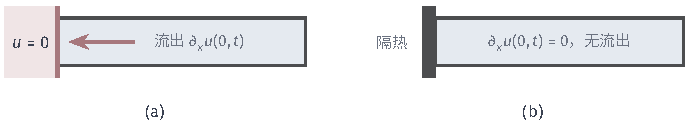
\includegraphics[width=112mm]{figures/06-differential-equations/02-partial-differential-equations/tikz/heat-boundary-meaning/figure.pdf}
  \caption{同一根暖棒左端的两种边界。(a)Dirichlet：端点接冰水，温度固定为$0$，红色箭头表示热量流出，流出率是$\partial_xu(0,t)$，由解决定。(b)Neumann：端点隔热（深灰），通量为零，温度由解决定。}
  \label{fig:heat-boundary-meaning}
\end{BookInlineFigure}

外法向通量是$-\partial_{\bm{n}}u$。所以Neumann数据$\partial_{\bm{n}}u=g>0$表示热量从外面进来，不是流出去。对无源的方程在$(0,1)$上积分，再用微积分基本定理，得到
\[
 \frac{\mathrm{d}}{\mathrm{d}t}\int_0^1u\,\mathrm{d}x=\partial_xu(1,t)-\partial_xu(0,t) .
\]
隔热时右端为零，总热量不变。接冰水时，只要棒内温度为正，左端斜率为正、右端斜率为负，右端小于零，总热量持续减少。

图~\ref{fig:heat-bump-two-boundaries}是同一个三角形在两种边界下的演化，公式下一节推出。短时间内两者几乎一样，因为中段还没有“听到”端点的消息。随后分歧变大：接冰水的鼓包整体下沉到零，隔热的鼓包摊平到平均温度$1/4$。

\begin{BookInlineFigure}
  \centering
  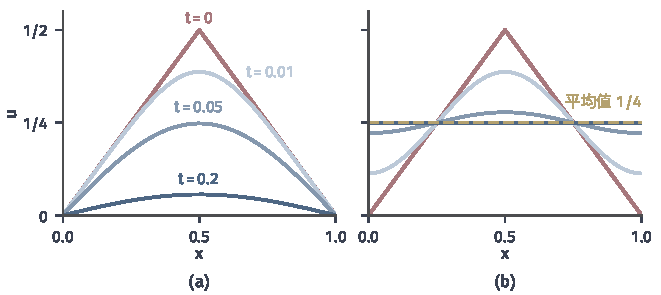
\includegraphics[width=112mm]{figures/06-differential-equations/02-partial-differential-equations/matplotlib/heat-bump-two-boundaries/figure.pdf}
  \caption{三角形初值（红）的演化，蓝色由浅到深为$t=0.01,0.05,0.2$。(a)两端$u=0$。(b)两端$\partial_xu=0$，黄色虚线是初值的平均值$1/4$，$t=0.2$的曲线已与它重合。}
  \label{fig:heat-bump-two-boundaries}
\end{BookInlineFigure}

图~\ref{fig:heat-spacetime-boundaries}把同样的解画在时空平面上。左图的红色竖边表示温度被固定，颜色向上逐渐褪成白色；右图的虚线竖边表示绝热，颜色褪成均匀的浅蓝，总量保留了下来。

\begin{BookInlineFigure}
  \centering
  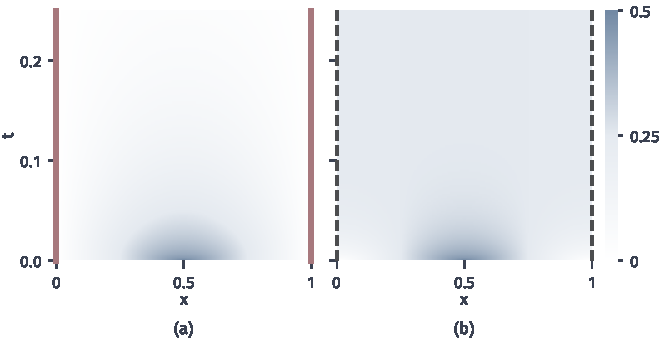
\includegraphics[width=112mm]{figures/06-differential-equations/02-partial-differential-equations/matplotlib/heat-spacetime-boundaries/figure.pdf}
  \caption{三角形初值解的时空温度图，颜色由白到蓝表示温度由$0$到$0.5$，两图色阶相同。(a)两端固定为$0$（红边）。(b)两端无通量（深灰虚边）。}
  \label{fig:heat-spacetime-boundaries}
\end{BookInlineFigure}

把两种条件并列，见表~\ref{tab:heat-boundary-compare}。此外还有介于两者之间的Robin条件$\partial_{\bm{n}}u+\beta u=0$（$\beta>0$），它说流出量正比于端点与环境的温差；$\beta\to0$接近隔热，$\beta\to\infty$接近固定温度。

\begin{BookInlineTable}
  \centering
  \caption{两种齐次边界条件的比较，数值取自三角形初值，$t=0.1$。}
  \label{tab:heat-boundary-compare}
  \begin{tabular}{lll}
    \toprule
    & 固定温度$u=0$ & 无通量$\partial_{\bm{n}}u=0$\\
    \midrule
    规定的量 & 端点温度 & 端点通量\\
    由解决定的量 & 端点通量 & 端点温度\\
    无源时总热量 & 减少 & 不变\\
    $t=0.1$的总热量 & $0.0962$ & $0.2500$\\
    $t=0.1$的中点温度 & $0.1511$ & $0.2539$\\
    \bottomrule
  \end{tabular}
\end{BookInlineTable}
